\chapter{提供サービスの考案プロセス}

\section{プロセス概要}
本プロジェクトの提供サービス考案までのプロセスは、大きく4つに分かれる。1つ目は、フィールドワークである。実際に函館を見て回り、街にある課題を探した。2つ目はブレインストーミングとKJ法(以下BSKJ法)である。フィールドワークで感じたことや、これまでの自身の体験をもとに函館の街に存在する課題を割り出し、それらをグルーピングした。3つ目はオープン・スペース・テクノロジー(以下OST)である。OSTを通してBSKJ法で出てきた課題やそれを解決する方法について議論し、アイデアを鮮明にした。4つ目はブラッシュアップである。BSKJ法やOSTを通して出たアイデアをより深堀りし、必要性や新規性などを考慮し、アイデアのブラッシュアップをおこなった。その他にもプロジェクトのロゴの制作や、ビーコンが使われたサービスを考案するにあたって必要な情報を入手する事前調査などの内容も説明する。
\bunseki{宮田悠冶}

\section{フィールドワーク}

\subsection{事前調査}
函館やその周辺の地域に存在する問題や課題を調査し、把握するためにフィールドワークをおこなった。はじめに、函館の地域を大きく5つに分け、「五稜郭」「赤川・美原・昭和・富岡」「函館駅・西部地区」「七飯・北斗」「空港・湯の川」の5地域のイメージを、ブレインストーミングをおこなって書き出した。そして、書き出した各イメージについて様々な視点からグルーピングをおこない、実地調査をおこなう際に注目する点を確認した。その後、各地域の実地調査をおこなう3人1組のグループを編成し、実地調査をおこなった。

\bunseki{平山翔真}

\subsection{フィールドワークに関するレクチャー}
フィールドワークの実施にあたり、40分ほどの動画にて南部美砂子先生よりフィールドワークについてのレクチャーを受けた。レクチャーでは、まずフィールドワークとはどのようなものなのかという説明があった。ただ街を歩いて見たり聞いたりするだけではなく、情報を得て整理し、考えて結論を出し、他者に伝達して行動することが大事であると学んだ。次に、COVID-19の影響の下でのフィールドワークについての説明があった。COVID-19の影響でフィールドに行けないということではなく、このCOVID-19が蔓延しているという環境そのものがフィールドであると学んだ。また、フィールドワークは目的ではなく手段の一つであり、フィールドワークの目的の一つは他者の合理性の理解であるということを学んだ。最後に、フィールドワーカーとしてのあり方についての説明があった。調査者は基本的に特権的存在であり、迷惑な侵入者という意識を持って調査をおこなうべきであるということや、守秘義務や匿名性、調査の説明や同意などに注意するべきであるということを学んだ。

\bunseki{平山翔真}

\subsection{実地調査}
実地調査は、プレ調査した後に本調査をおこなった。プレ調査では、函館山で6月19日に実施した。本調査では、2.2.1節で述べた5つの地区で5つのグループに分かれて6月21日に実施した。ただし、COVID-19感染への対策として体調の管理やマスク着用必須、人混みや他人との接触・会話を避けるなどに注意することとした。五稜郭地区では、五稜郭公園、五稜郭タワー、五稜郭交差点地下横断歩道、千代台公園、JR五稜郭駅、函館市中央図書館、六花亭で主に調査をおこなった。赤川・美原・昭和・富岡地区では、四季の杜公園、笹流ダム、四稜郭、住宅街で主に調査をおこなった。函館駅・西部地区では、函館駅周辺、金森赤レンガ倉庫、朝市、西部地区で主に調査をおこなった。七飯・北斗地区では、男爵ラウンジ、なないろ・ななえ、新函館北斗駅、大沼公園、山川牧場で主に調査をおこなった。空港・湯の川地区では、あいす118、函館空港、トラピスチヌ修道院、香雪園、植物園、函館公園、十字街で主に調査をおこなった。また、各グループでSlackにチャンネルを作成し、調査をおこないながら写真や文章で情報をリアルタイムで共有した。

\bunseki{平山翔真}

\subsection{振り返り}
調査で得た情報をまとめて他の班と共有するため、各グループでフィールドワーク中に気づいた点について、Google Jamboardに写真や付箋を用いて書き出した。そして、書き出した写真や付箋をグループ分けした。その後、全グループでZoomに集まり、各グループのGoogle Jamboardを見せながら結果を共有した。プレ調査では、函館山を訪れた。調査の結果、展望台やロープウェイにはビーコンが設置されていること、山でもGPSが利用できること、登山道の一部ではソーシャルディスタンスが保ちにくいこと、登山道が多く、迷いやすいことなどがわかった。本調査では、2.2.1節で述べた5つの地区を訪れた。調査の結果、五稜郭や函館駅、湯の川周辺などの主に観光地で、時短営業や観光客の減少などのCOVID-19の影響が見られること、夏にマスクを着用しながら歩き回るのはつらいこと、函館駅・西部地区では多くの撮影スポットがあること、公園では年配の方が多いことなどがわかった。

\bunseki{平山翔真}

\begin{figure}[htbp]
    \begin{center}
    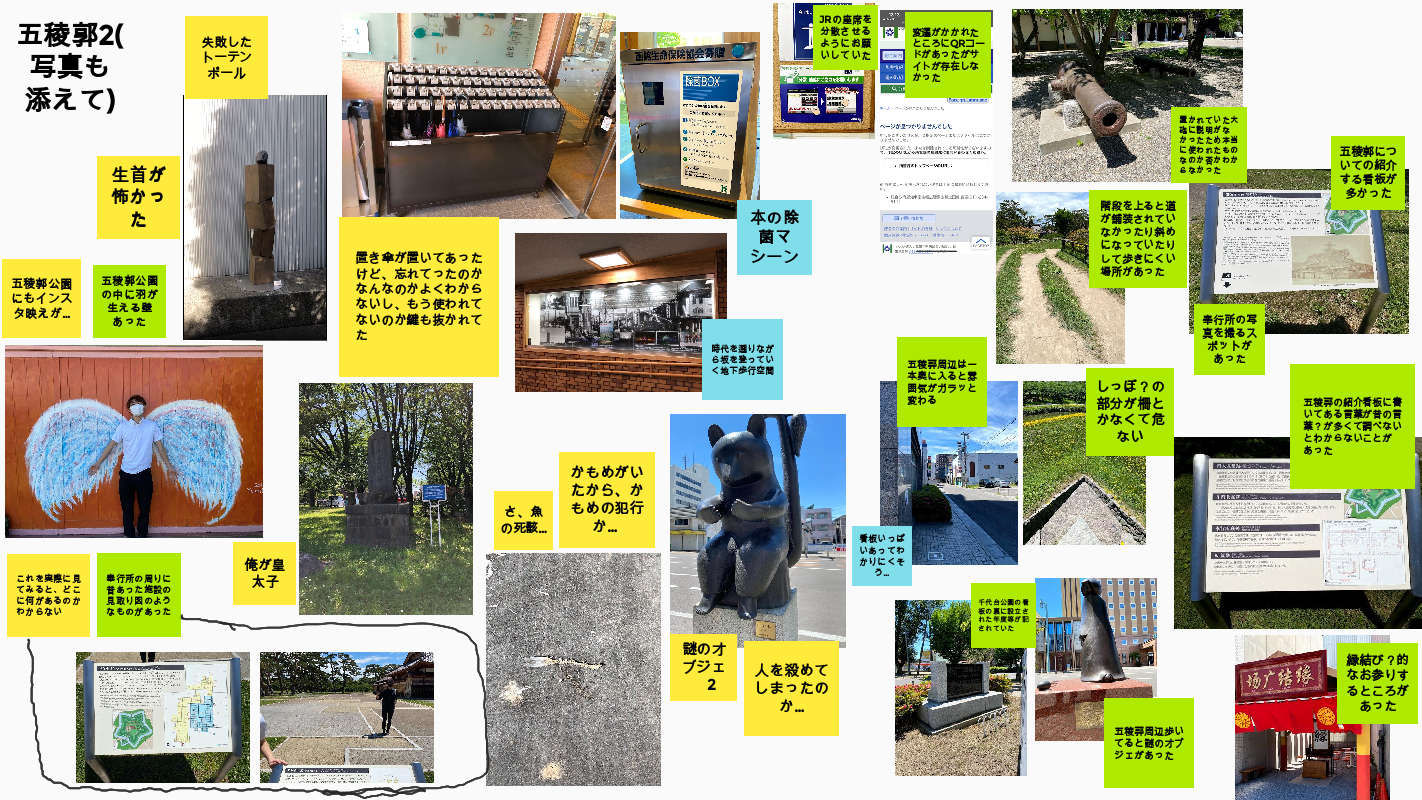
\includegraphics[width=8cm]{images/FW1.png}
    \end{center}
    \caption{フィールドワーク振り返り1}
    \label{fig:furikaeri1}
\end{figure}

\begin{figure}[htbp]
    \begin{center}
    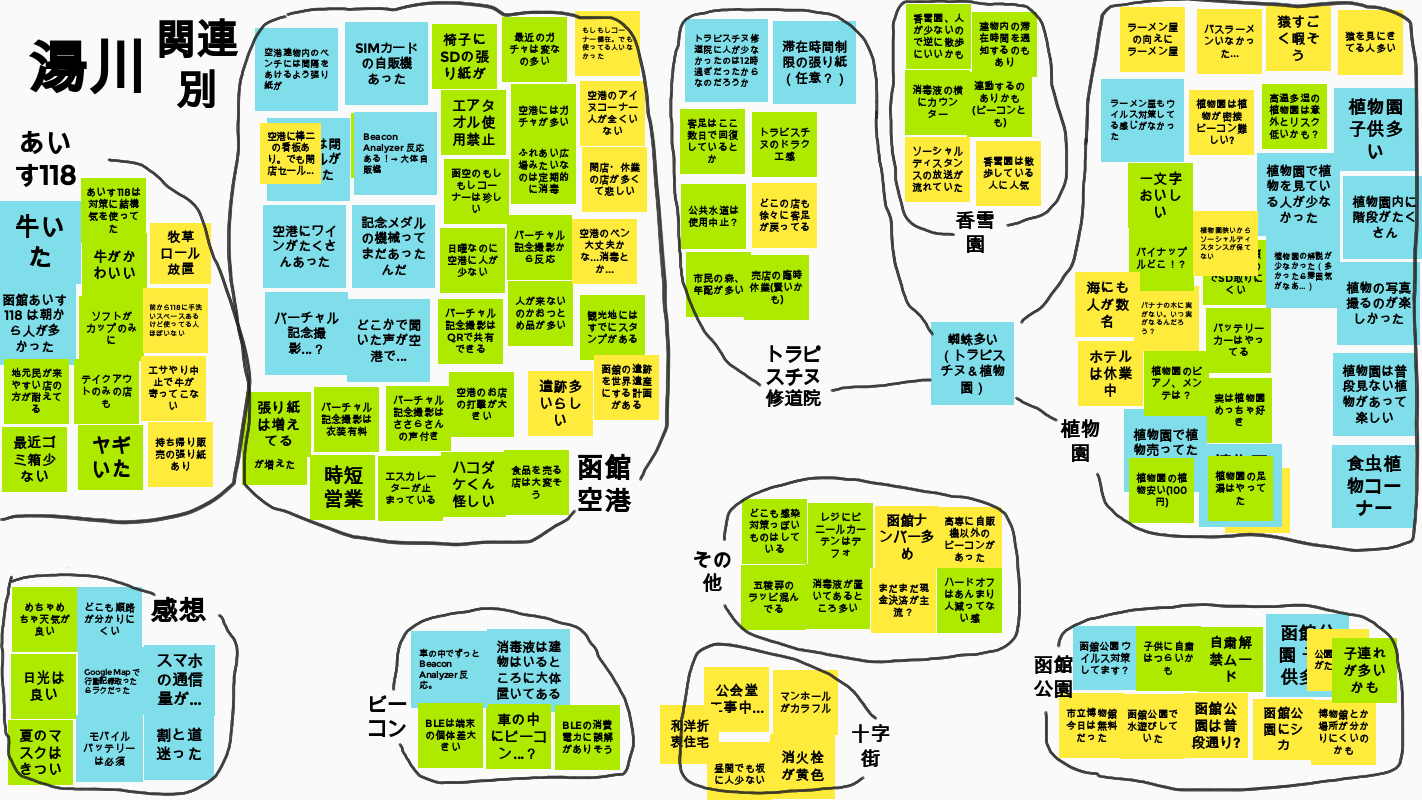
\includegraphics[width=8cm]{images/FW2.png}
    \end{center}
    \caption{フィールドワーク振り返り2}
    \label{fig:furikaeri2}
\end{figure}


\section{サービスの考察}

\subsection{BSKJ法(ブレインストーミングKJ法)}
フィールドワーク後、ブレインストーミングを踏まえてBSKJ法をおこなった。BSKJ法とは、思いつく限り多くの量のアイデアを出すというブレインストーミングと、それらを付箋等にアウトプットして得られたアイデアを整序しグルーピングをおこなうKJ法と組み合わせた方法である。今回は4人1グループを3グループ作り、フィールドワークの共有結果を見ながら、Google Jamboardで付箋にアイデアを書いて、貼り付けをおこない、それぞれのグループごとに様々な観点からグルーピングをおこなった。また、KJ法に関しては、OSTをおこなった後、アイデアをまとめるときに用いることで、アイデアの絞りこみを円滑におこなうことができた。
\bunseki{山本雄平}

\subsection{ハッカソン方式}
ハッカソンはハックとマラソンを掛け合わせた造語で、チームを作成し、短期間でサービスやシステム、アプリケーションを開発し、成果を競うイベントの一種である。私たちはこのハッカソンを2回のアイデア出しに用いた。以下ハッカソン方式と呼ぶ。1回目は、4人1グループを作成し、90分の時間制限を設けてアイデアを出しをおこなった。2回目は参加者が順番に出題し、5分の時間制限を設けてお題に沿ったアイデア出しをおこなった。この方式ではそれぞれがアイデアの絵を描いてメンバーにイメージを共有しながら進めていった。
\bunseki{山本雄平}

\subsection{OST(オープンスペーステクノロジー)}
BSKJ法とハッカソン方式をおこなった後に、関心のあるテーマについて深く、創造的に考える時間をもつことができる方法であるOSTを実施した。今回はBSKJ法3グループ、ハッカソン方式1グループでそれぞれ部屋を作成し、プロジェクトメンバーは興味のあるアイデアを出している部屋に移動して、議論をおこなった。OSTを通じて、各々が興味のあるアイデアについて深めることや、他グループのアイデアの発想を持ち帰り、考案したアイデアをより具体的なものにすることができた。OSTではアイデアによって議論が進んだものと、それほど議論がなされなかったものとで、アイデアの選定ができるので、その後のアイデアの絞りこみやブラッシュアップにつなげることができた。
\bunseki{山本雄平}

\subsection{アイデアのブラッシュアップ}
KJ法ですべての班のアイデアのグルーピングをおこなった結果からブラッシュアップをおこなうにあたりアイデアの絞り込みをおこなった。メンバーは1~4点の計10点を持ち点として各々が興味のあるアイデアに投票をおこない、絞りこみをおこなった。その結果、中間発表の時点では「お店とビーコン」「観光」「隠れスポット」「施設とビーコン」の4つの項目に絞ることができた。その後、これらのアイデアに3~4人割り振って、アイデアのブラッシュアップをおこなった。各グループでのブラッシュアップの内容をesaにまとめた後、メンバー、TA、先生を交えてレビューをおこない、それを参考にして、さらにブラッシュアップをおこなっていった。今後は中間発表時のアイデアと夏季休暇中のアイデア出しでのアイデアを「サービスの函館らしさ」「ビーコンである理由」「サービスの必要性」「サービスの新規性」「サービスの不変的な魅力」の5つの観点でブラッシュアップをおこない、最終的なアイデアを出していく。
\bunseki{山本雄平}

\subsection{テーマの決定}
現在、テーマの決定作業の途中であり、「サービスの函館らしさ」「ビーコンである理由」「サービスの必要性」「サービスの新規性」「サービスの不変的な魅力」の5つの観点で有力なアイデアは「俺を食ってくれぇ!」「函館のここ、おすすめかも」「函館を舞台にしたADV」「目の前のイベントは何?」の4つである。「俺を食ってくれぇ!」は、函館の海産物に焦点を当てたサービスで、海産物の状態によって調理方法を提示してくれるもので、食品自体が自分の食われ方をアピールするというサービスである。「函館のここ、おすすめかも」は、アプリを付けたまま、函館の街を歩くことで、行動履歴をもとに、訪れた店との関連性や好みに合わせてお店を提案するというサービスである。「函館を舞台したADV」は函館を舞台にした物語を作成し、物語のキーとなる場所にビーコンを設置し、実際に聖地巡礼をかねて追加ストーリーなどがゲットすることを通じて、函館の魅力を発見できるサービスである。「目の前のイベントは何?」は函館はイベントが多く、目の前のイベントが何だか知りたいときに、ビーコンを設置することで、イベントのwebサイト閲覧やレビューをすることができるサービスである。これらのアイデアを主軸にして他のアイデアを統合し、最終的なテーマを決定する。
\bunseki{山本雄平}

\section{その他}
\subsection{ロゴ作成}
本プロジェクトでは、プロジェクトの特徴やイメージを表現するため、加えて議論の練習と、メンバー全員の一体感を生むために、今年度のプロジェクトのロゴを制作した。ロゴの制作には3週間の時間を要し、決定に至った。まずはじめに、メンバー全員がロゴ案を1案以上考案してロゴの発表会をおこない、それぞれの案についてレビューをおこなった。この段階ではそれぞれの案の良いところだけを伝える形式をとった。ここで受けたレビューと、他のメンバーのロゴデザインを参考に、各自ロゴの改善をし、2回目の発表会をおこなった。この発表会のレビューでは、良いところと改善点の指摘を含めたレビューをおこない、その後投票によって4つのロゴ案に絞り込んだ。このレビューをもとに、再度ロゴの改善をおこない3回目の発表会をおこなった。この発表会後、「サービスの函館らしさ」「ビーコンらしさ」を考慮したうえで、メンバー、TA、先生を交えて最終投票をおこなって今年度のロゴを決定した。その後、ロゴに関するワーキンググループを結成し、デザイン原案の改善をおこなった。ロゴデザインの最終版とロゴ使用に関するガイドラインを作成した。

\begin{figure}[htbp]
    \begin{center}
    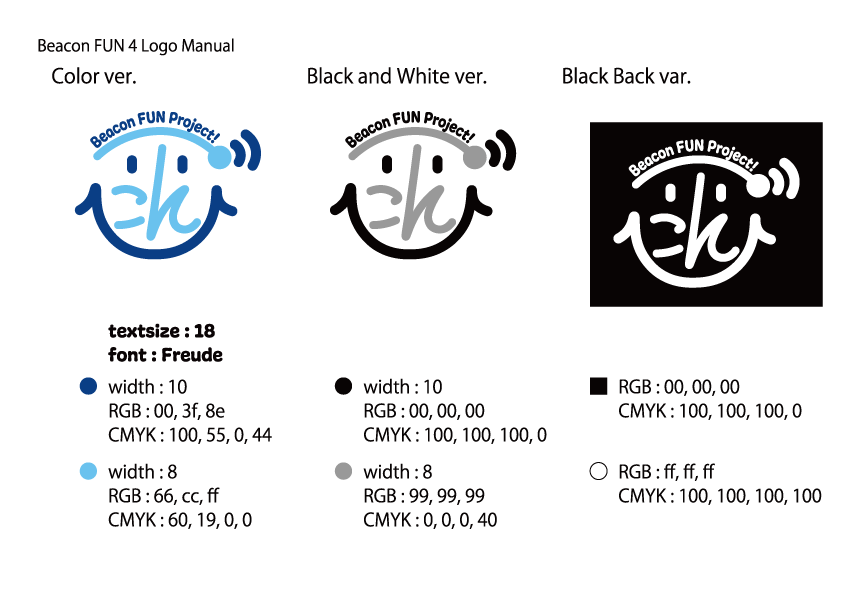
\includegraphics[width=14cm]{images/BeaconFUN4Logo_Manual.png}
    \end{center}
    \caption{ロゴガイドライン}
    \label{fig:LogoManual}
\end{figure}

\bunseki{伊藤直樹}

\subsection{ビーコンについての事前調査}
本プロジェクトではビーコンを使用した開発をおこなうために、ビーコンに関する知識を深める必要があると判断し、事前調査をおこなった。事前調査は「近接・位置測位」「GPSとの機能・特性比較」「各種センサとの連携」「LINE Beacon」「適用事例」の5つの項目についておこなった。各項目にメンバーを3名ずつ割り振って調査をおこない、調査した内容を各グループスライドにまとめ、共有した。この事前調査によって、ビーコンの特徴や機能など、様々な知識を会得することができた。またこの調査は、アイデアにビーコンらしさを取り入れる点で非常に役立っている。
\bunseki{伊藤直樹}

\subsection{夏休み勉強会の実施計画}
本プロジェクトでは後期からの本格的な開発に向けて、夏休み勉強会を実施した。この勉強会について形式は特に決めず、自分の持っている知識や、夏季休暇中におこなったことをLT形式で発表したり、ライブコーディングなどをおこなった。自分の興味のあるプラットフォームの勉強会には積極的に参加してもらい、1人約1時間ほどの勉強会を、メンバー全員がそれぞれ2回おこなった。この勉強会を通じて、自分が開発に携わりたいプラットフォームについての知識が深められ、円滑に開発に進められることが期待される。
\bunseki{伊藤直樹}

\subsection{昨年度のサービス紹介}
昨年度の本プロジェクトでは、4つのサービスを開発した。1つ目は「去りし想ひを乗せゆきて」というサービスで、函館の市電から見えるノスタルジックな景色から、1人1句投稿して5人で短歌を作り上げるサービスである。2つ目は「みみうち」というサービスで、店の来店回数に応じて限定メニューの提案や、クーポンを配布してくれるサービスである。3つ目は「ゆまち」というサービスで、温泉を訪れた家族を含む男女が、互いに大浴場内の大まかな位置を把握することで、脱衣所に向かうタイミングを揃えられるようにするサービスである。4つ目は「函ライブ」というサービスで、キーボードの演奏をビーコンで配信し、演奏を聴きたい人のみアプリを通じて音楽を聴くことができるサービスである。以上4つが昨年開発されたサービスである。
\bunseki{伊藤直樹}
